\documentclass[oneside]{ausarbeitung}
\bibliography{latexlit}

\usepackage{hyperref}
\usepackage{tikz}

% ----------------------------------------------------------------------

\begin{document}

\selectlanguage{ngerman}

%--- Art der Arbeit
% Erlaubte Werte:
% Praxissemesterbericht, Projektbericht, Bachelorarbeit oder                                % Masterarbeit
\doctype{Projektbericht}

%--- Studiengang:
\depname{Medieninformatik}

\title{expressionviewer}

\author{Laurin Agostini}
\matrikelnr{60526}

\examinerA{Prof.~Dr.~Winfried~Bantel}
\date{25. November 2019}

%--- Titelseite Anzeigen
\maketitle
\cleardoublepage

%---
\pagenumbering{roman}
\setcounter{page}{1}


%--- Eidesstattliche Erklärung anzeigen
\makeaffirmation
\cleardoublepage

%---
\chapter*{Kurzfassung}
\addcontentsline{toc}{chapter}{Kurzfassung}

Ziel der Kurzfassung ist es, einen (eiligen) Leser zu informieren, so 
dass dieser entscheiden kann, ob der Bericht für ihn hilfreich ist oder 
nicht (neudeutsch: Management Summary). Die Kurzfassung gibt daher eine 
kurze Darstellung

\begin{itemize}
  \item des in der Arbeit angegangenen Problems
  \item der verwendeten Methode(n)
  \item des in der Arbeit erzielten Fortschritts.
\end{itemize}

Dabei sollte nicht auf die Struktur der Arbeit eingegangen werden, also 
Kapitel~\ref{cha:grundlagen} etc. denn die Kurzfassung soll ja gerade 
das Wichtigste der Arbeit vermitteln, ohne dass diese gelesen werden muss. Eine Kapitelbezogene Darstellung sollte sich in Kapitel~%
\ref{cha:einleitung} unter Vorgehen befinden.

Länge: Maximal 1 Seite.

%-----------------------------------------------------------------------
\cleardoublepage
\addcontentsline{toc}{chapter}{Inhaltsverzeichnis}
\tableofcontents

%---
\addcontentsline{toc}{chapter}{Abbildungsverzeichnis}
\listoffigures

%---
\addcontentsline{toc}{chapter}{Tabellenverzeichnis}
\listoftables

%---
\chapter*{Abkürzungsverzeichnis}
\addcontentsline{toc}{chapter}{Abkürzungsverzeichnis}
\begin{acronym}[ANSI C / C89]  % Längstes Kürzel in der nachfolgenden
                       % Liste um die Breite der Spalte für die
                       % Abkürzungen zu bestimmen.

%% Eintrag: \acro{Referenzname}[Kürzel]{Langform}
%% Im Text wird die Abkürzung dann mit \ac{Referenzname} benutzt.
\acro{bsp}[Bsp.]{Beispiel}
\acro{rup}[RUP]{Ratified Unified Process}
\end{acronym}
%---
\cleardoublepage
\pagenumbering{arabic}
\setcounter{page}{1}

% ----------------------------------------------------------------------
\chapter{Einleitung}
\label{cha:einleitung}

Die Einleitung dient dazu, beim Leser Interesse für die Inhalte 
Praxissemesterberichts zu wecken, die behandelten Probleme aufzuzeigen 
und die zu ihrer Lösung entwickelten Konzepte zu beschreiben.

\section{Motivation}
\label{sec:motivation}

In der Motivation wird dargestellt, welche Bedeutung die im 
Praxissemester zu entwickelnden Lösungen für das betreuende Unternehmen 
haben. Es wird beispielsweise aufzeigt, in welches Produkt sie eingehen, 
welcher Ablauf verbessert werden soll etc.

\begin{figure}[htbp]
  \centering
  \includegraphics[width=0.8\textheight]{images/tree.pdf}
  \caption{Beispielausgabe in Tikz}
  \label{fig:motivation}
\end{figure}

\section{Problemstellung und -abgrenzung}
\label{sec:problemstellung}

Die Problemstellung dient dazu, das zu lösende Problem klar zu 
definieren und abzugrenzen. Der Praktikant soll ein klares Verständnis 
des zu lösenden Problems haben. Insbesondere soll auch verhindert 
werden, dass zu viele Probleme gleichzeitig angegangen werden. Eine 
Negativabgrenzung verhindert, dass beim Leser später nicht erfüllte 
Erwartungen geweckt werden.

\section{Ziel der Arbeit}
\label{sec:ziel}

Es soll ein Werkzeug für Programmieranfänger erstellt werden, womit diese einen \hyperref[sub:c89]{C89 / ANSI C} \hyperref[sub:expression]{Ausdruck} analysieren können. Das Werkzeug soll den \hyperref[sub:expression]{Ausdruck} in einen \hyperref[sub:syntax_tree]{Syntaxbaum} mit Typinformationen umwandeln, d. h. für jeden Knoten im Syntaxbaum soll der Datentyp und der aktuelle Wert angezeigt werden. Außerdem sollen Fehler und ihre Folgen im Syntaxbaum ausdrücklich markiert und beschrieben werden.

\section{Vorgehen}
\label{sec:vorgehen}

Nachdem mit Problemstellung und Ziel gewissermaßen Anfangs- und Endpunkt 
des Praktikums beschrieben sind, wird hier der zur Erreichung des Ziels 
eingeschlagene Weg vorgestellt. Dazu werden typischerweise die folgenden 
Kapitel und ihr Beitrag zur Erreichung des Ziels der Arbeit kurz 
beschrieben. Die folgenden Kapitel sind ein – möglicher – Aufbau, 
Abweichungen können durchaus notwendig sein. Zur Darstellung des 
Vorgehens ist eine grafische Darstellung sinnvoll, bei der die einzelnen 
Lösungsschritte und ihr Zusammenhang dargestellt werden. Ein Beispiel 
hierfür findet sich in Abbildung \ref{fig:1}.


% ---
\chapter{Grundlagen}
\label{cha:grundlagen}

In diesem Kapitel das für das Praktikum relevante Grundlagenwissen 
dargestellt. Der Praktikant soll hierzu das ihm durch Vorlesungen 
bekannte, bzw. durch Recherchen vertiefte theoretische Wissen 
darstellen, das für die Lösung der im Praktikum gestellten Probleme 
notwendig ist.

Dabei ist darauf zu achten, nur solche Inhalte in das Grundlagenkapitel 
aufzunehmen, die später auch verwendet werden (Problembezogenheit). 
Ebenso ist auf eine ausreichend tiefe und vollständige Darstellung der 
Grundlagen zu achten.

Für die Erstellung des Literaturverzeichnisses 
wird das Werkzeug JabRef\autocite{JabRef:JabRef} verwendet. 

Sie können aber auch das Werkzeug Citavi\autocite{SAS:Citavi} benutzen
und dort nach \textsc{Bib}\TeX{} exportieren.

\section{Programmiersprachen}
\label{sec:prog_langs}

\subsection{C89 / ANSI C}
\label{sub:c89}
Erster offizieller Standard der C-Programmiersprache, der 1989 veröffentlicht wurde. Wird als Grundlage für die zu verarbeitenden Ausdrücke genommen.

\subsection{C99}
\label{sub:c99}
Zweiter offizieller Standard der C-Programmiersprache, 1999 veröffentlicht. Mit diesem Standard wurde das Kommandozeilenprogramm der Projektarbeit geschrieben.

\section{Compilerbau}

\subsection{Ausdruck}
\label{sub:expression}
Eine Kombination von Konstanten, Variablen, Funktionsaufrufen und Operationen die einen Wert liefert.
Ausdrücke an sich haben keinen direkten Einfluss auf den Programmfluss, anders wie Verzweigungen(if) oder Schleifen(while, for). <<TODO>>

\subsection{Syntaxbaum}
\label{sub:syntax_tree}
Hierarchische Darstellung der Zergliederung des zu verarbeitenden Quellcodes.

\begin{figure}[htbp]
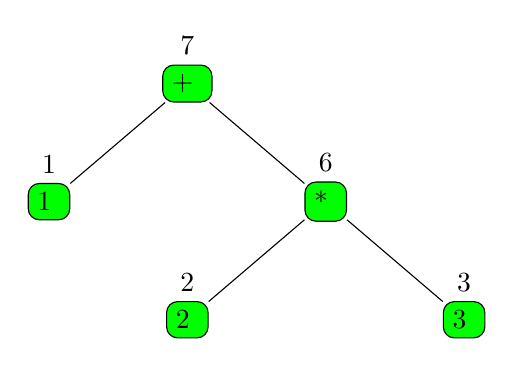
\begin{tikzpicture}[sibling distance=10em, every node/.style = {shape=rectangle, rounded corners, draw, align=center}]]
\node[fill=green, label={7}] { + }
child { node[fill=green, label={1}] { 1 }}
child { node[fill=green, label={6}] { * }
 child { node[fill=green, label={2}] { 2 } }
 child { node[fill=green, label={3}] { 3 } }
}
;
\end{tikzpicture}
\centering
\caption{Syntaxbaum für den Ausdruck \textit{1 + 2 * 3}}
\label{fig:example_syntax_tree}
\end{figure}

\subsection{Scanner}
\label{sub:scanner}
Ein Werkzeug, das den Eingabetext in Tokens umwandelt. Kann Fehler in der Zeichenabfolge innerhalb eines Tokens finden, aber nicht in der Abfolge mehrerer Tokens.


\subsection{Parser}
\label{sub:parser}
Ein Werkzeug, das die vom Scanner generierte Tokenabfolge einliest und validiert. Kann für jede Tokenkombination eine Aktion auslösen, wie zum Beispiel das Hinzufügen eines Knoten im Syntaxbaum.

%---
\chapter{Problemanalyse}
\label{cha:problemanalyse}

Die Analyse des zu lösenden Problems ist Grundlage für jedes 
ingenieurmäßige Vorgehen. Daher soll in diesem Kapitel das zu lösenden 
Problem auf Basis des im Grundlagenkapitel aufbereiteten Wissens 
analysiert werden. Hierzu ist insbesondere notwendig zu klären, wie sich 
das Gesamtproblem in Teilprobleme zerlegen lässt und welche 
Abhängigkeiten zwischen diesen bestehen.

Bei Software-Projekten befindet sich an dieser Stelle typischerweise die 
Anforderungsanalyse des \ac{rup}.

%---
\chapter{Implementierung}
\label{cha:implementierung}

Die Grundarchitektur des Lösungskonzeptes besteht aus einer klassischen Unterteilung in Front- und Backend. Das Frontend ist für die Datenabfrage und die Darstellung zuständig. Im Backend wiederum steckt die eigentliche Logik des Programms. Da das eigentliche Backend auch als eigenständiges Kommandozeilenprogramm funktionieren soll, wurde die Kommunikation mit dem Frontend auf ein Backend-Interface ausgelagert, die das Kommandozeilenprogramm auf dem Server aufruft und die Resultate zurück an das Frontend schickt.

\begin{figure}
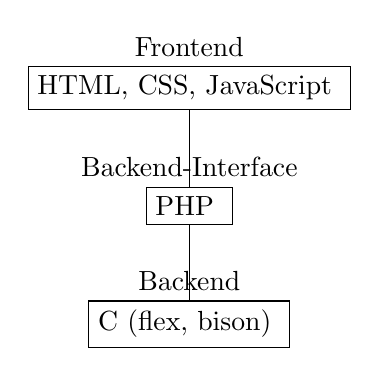
\begin{tikzpicture}[sibling distance=10em, every node/.style = {shape=rectangle, draw, align=center}]]
\node[fill=white, label={Frontend}] { HTML, CSS, JavaScript }
child { node[fill=white, label={Backend-Interface}] { PHP } 
 child { node[fill=white, label={Backend}] { C (flex, bison) } }
}
;
\end{tikzpicture}
\centering
\caption{Grundarchitektur}
\label{fig:architecture}
\end{figure}

\section{Frontend}
\label{sec:frontend}
Das gesamte Frontend besteht aus einer HTML-, einer CSS- und zwei JavaScript-Dateien (eine davon ist die zur Darstellung des Syntaxbaum verwendete \href{https://d3js.org}{D3.js} Bibliothek). Die HTML und CSS Dateien sind je unter 50 Quellcodezeilen lang und somit sehr trivial gehalten. In der eigenen JavaScript-Datei werden die Eingaben des Benutzers ausgelesen, formatiert und dann an das Backend geschickt. Die Antwort wird wiederum verwendet um den resultierenden Syntaxbaum zu zeichnen.

\section{Backend-Interface}
\label{sec:backend_interface}
Das Backend-Interface besteht aus einer einzigen PHP-Datei, die im Grunde nichts anderes macht, als das eigentliche Backend mit den Parametern aus der Anfrage des Frontends aufzurufen und die Ergebnisse formatiert wieder ans Frontend zurückzuschicken.

\section{Backend}
\label{sec:backend}
Der Großteil der Arbeit ist in das, auch eigenständig als Kommandozeilenprogramm benutzbare, Backend geflossen. Dieses nimmt grundlegend einen Ausdruck und eine Reihe von Symboldefinitionen(die auch leer sein kann) entgegen und gibt den resultierenden Syntaxbaum in einem der Formate (JSON oder tex) auf der Standardausgabe aus. Alternativ kann die Ausgabe auch direkt in eine Datei geschrieben werden. Für die Generierung des \hyperref{sub:scanner}{Scanners} wurde hierbei Flex und für die Generierung des \hyperref{sub:parser}{Parsers} Bison verwendet.

Bei Software-Projekten besteht dieses Kapitel typischerweise aus den 
Phasen Implementierung \& Test im \ac{rup}.

%---
\chapter{Evaluierung}

Aufgabe des Kapitels Evaluierung ist es, in wie weit die Ziele der 
Arbeit erreicht wurden. Es sollen also die erreichten Arbeitsergebnisse 
mit den Zielen verglichen werden. Ergebnis der Evaluierung kann auch 
sein, das bestimmte Ziele nicht erreicht werden konnten, wobei die 
Ursachen hierfür auch außerhalb des Verantwortungsbereichs des 
Praktikanten liegen können.

%---
\chapter{Zusammenfassung und Ausblick}
\label{cha:zusammenfassung}

\section{Erreichte Ergebnisse}
\label{sec:ergebnisse}

Die Zusammenfassung dient dazu, die wesentlichen Ergebnisse des 
Praktikums und vor allem die entwickelte Problemlösung und den 
erreichten Fortschritt darzustellen. (Sie haben Ihr Ziel erreicht und 
dies nachgewiesen).

\section{Ausblick}
\label{sec:ausblick}

\subsection{Erweiterbarkeit der Ergebnisse}
\label{sub:erweiterbarkeit}

\subsubsection{Hinzufügen weiterer primitiver Datentypen (char, long, bool, float, etc.)}
Prinzipiell dürfte das Hinzufügen weiterer primitiver Datentypen keine großen Probleme bereiten, jedoch müsste so gut wie jeder \textit{Node} angepasst werden, um mit dem neuen Datentyp umgehen zu können.
\begin{itemize}
\item{Schwierigkeit: Niedrig}
\item{Aufwand: Mittel}
\end{itemize}
\subsubsection{Felder als Datentyp}
Für die Implementierung von Feldern müsste auf jeden Fall die Symbol Tabelle überarbeitet werden. Ein einfacher Weg wäre hier zum Beispiel die Definition von 10 \textit{int}-Symbolen mit automatisch generierten Namen für ein \textit{int}-Feld der Größe 10. Wenn wir dann nur von einfachen Lese- und Schreiboperationen mithilfe des Index-Operators \textit{[]} auf die einzelnen Datenfelder ausgehen, würde sich der Aufwand bei den \textit{Nodes} hier wohl auf eine Anpassung des Lese-\textit{Nodes} von Variablen und dem Zuweisungs-\textit{Nodes} beschränken.
\begin{itemize}
\item{Schwierigkeit: Niedrig}
\item{Aufwand: Niedrig}
\end{itemize}
\subsubsection{Zeiger als Datentyp}
Da man Variablen bisher nur konstante Werte und keine Ausdrücke  oder andere Variablen zuweisen kann ist der Nutzen für Zeiger noch sehr begrenzt. Zur Lösung des Problems müssten die Werte der Variablendefinitionen auch als Ausdrücke ausgewertet werden. Um den Zugriff über die Adresse einer Variable zu erlauben, könnte die Symbol Tabelle wahrscheinlich relativ einfach angepasst werden.
\begin{itemize}
\item{Schwierigkeit: Mittel}
\item{Aufwand: Hoch}
\end{itemize}
\subsubsection{Zeigerarithmetik}
Zeigerarithmetik (Berechnung der Zeigeradresse inklusive Inkrement und Dekrement) benötigt eine Emulation des Speichers und somit grundlegende Änderungen an mehreren Basissystemen (zum Beispiel an der Symbol Tabelle).
\begin{itemize}
\item{Schwierigkeit: Hoch}
\item{Aufwand: Hoch}
\end{itemize}
\subsubsection{Hinzufügen von Anweisungen (Verzweigungen, Schleifen)}
?
\begin{itemize}
\item{Schwierigkeit: ?}
\item{Aufwand: ?}
\end{itemize}
\subsubsection{Bearbeiten des Syntaxbaums...}
Das Bearbeiten des Syntaxbaums im Frontend müsste mit der \href{https://d3js.org}{D3.js}-Bibliothek möglich sein, jedoch habe ich mich im Rahmen dieser Arbeit nicht weiter damit befasst.
\begin{itemize}
\item{Schwierigkeit: Nicht einschätzbar}
\item{Aufwand: Nicht einschätzbar}
\end{itemize}
\subsubsection{...und Generieren des entstandenen \textit{C}-Ausdrucks}
Das Generieren des \textit{C}-Ausdrucks aus einem Syntaxbaum besteht größtenteils nur aus Textkonkatenation der Namen der einzelnen Knoten. Bei einzelnen Knoten (zum Beispiel der ternäre Operator oder Funktionen mit Parametern) ist etwas mehr Aufwand von Nöten.
\begin{itemize}
\item{Schwierigkeit: Niedrig}
\item{Aufwand: Niedrig}
\end{itemize}

\subsection{Übertragbarkeit der Ergebnisse}
\label{sub:uebertragbarkeit}

%-----------------------------------------------------------------------
\appendix

%---
\printbibliography

%---
\chapter{Anhang A}

%---
\chapter{Anhang B}


\end{document}